\clearpage
\section{3 ДАЛЬНЕЙШЕЕ РАЗВИТИЕ РЕАЛИЗАЦИИ}
В ходе реализации упрощённой системы были выявлены следующие технические проблемы, на решение которых необходимо обратить внимание при реализации полной версии:
\begin{itemize}
    \item задача разбиения графа;
    \item ограничение размера мешлетов;
    \item оптимизация структуры мешлетов;
    \item оптимизация отрисовки треугольников;
    \item организация параллельного спуска по графу;
    \item организация параллельной децимации.
\end{itemize}

\subsection*{Задача разбиения графа}
Основной проблемой при реализации является задача разбиения графа.
Эта задача является NP-трудной, для неё не доказано даже вхождение в класс NP.
Из-за этого алгоритмы в библиотеке METIS, как и любые приемлемые алгоритмы в любой другой библиотеке, вычисляют только приближение решения.
Это приводит к значительной неравномерности разбиения, как на рисунке~\ref{fig:sphere-0}.
\begin{figure}[H]
    \centering
    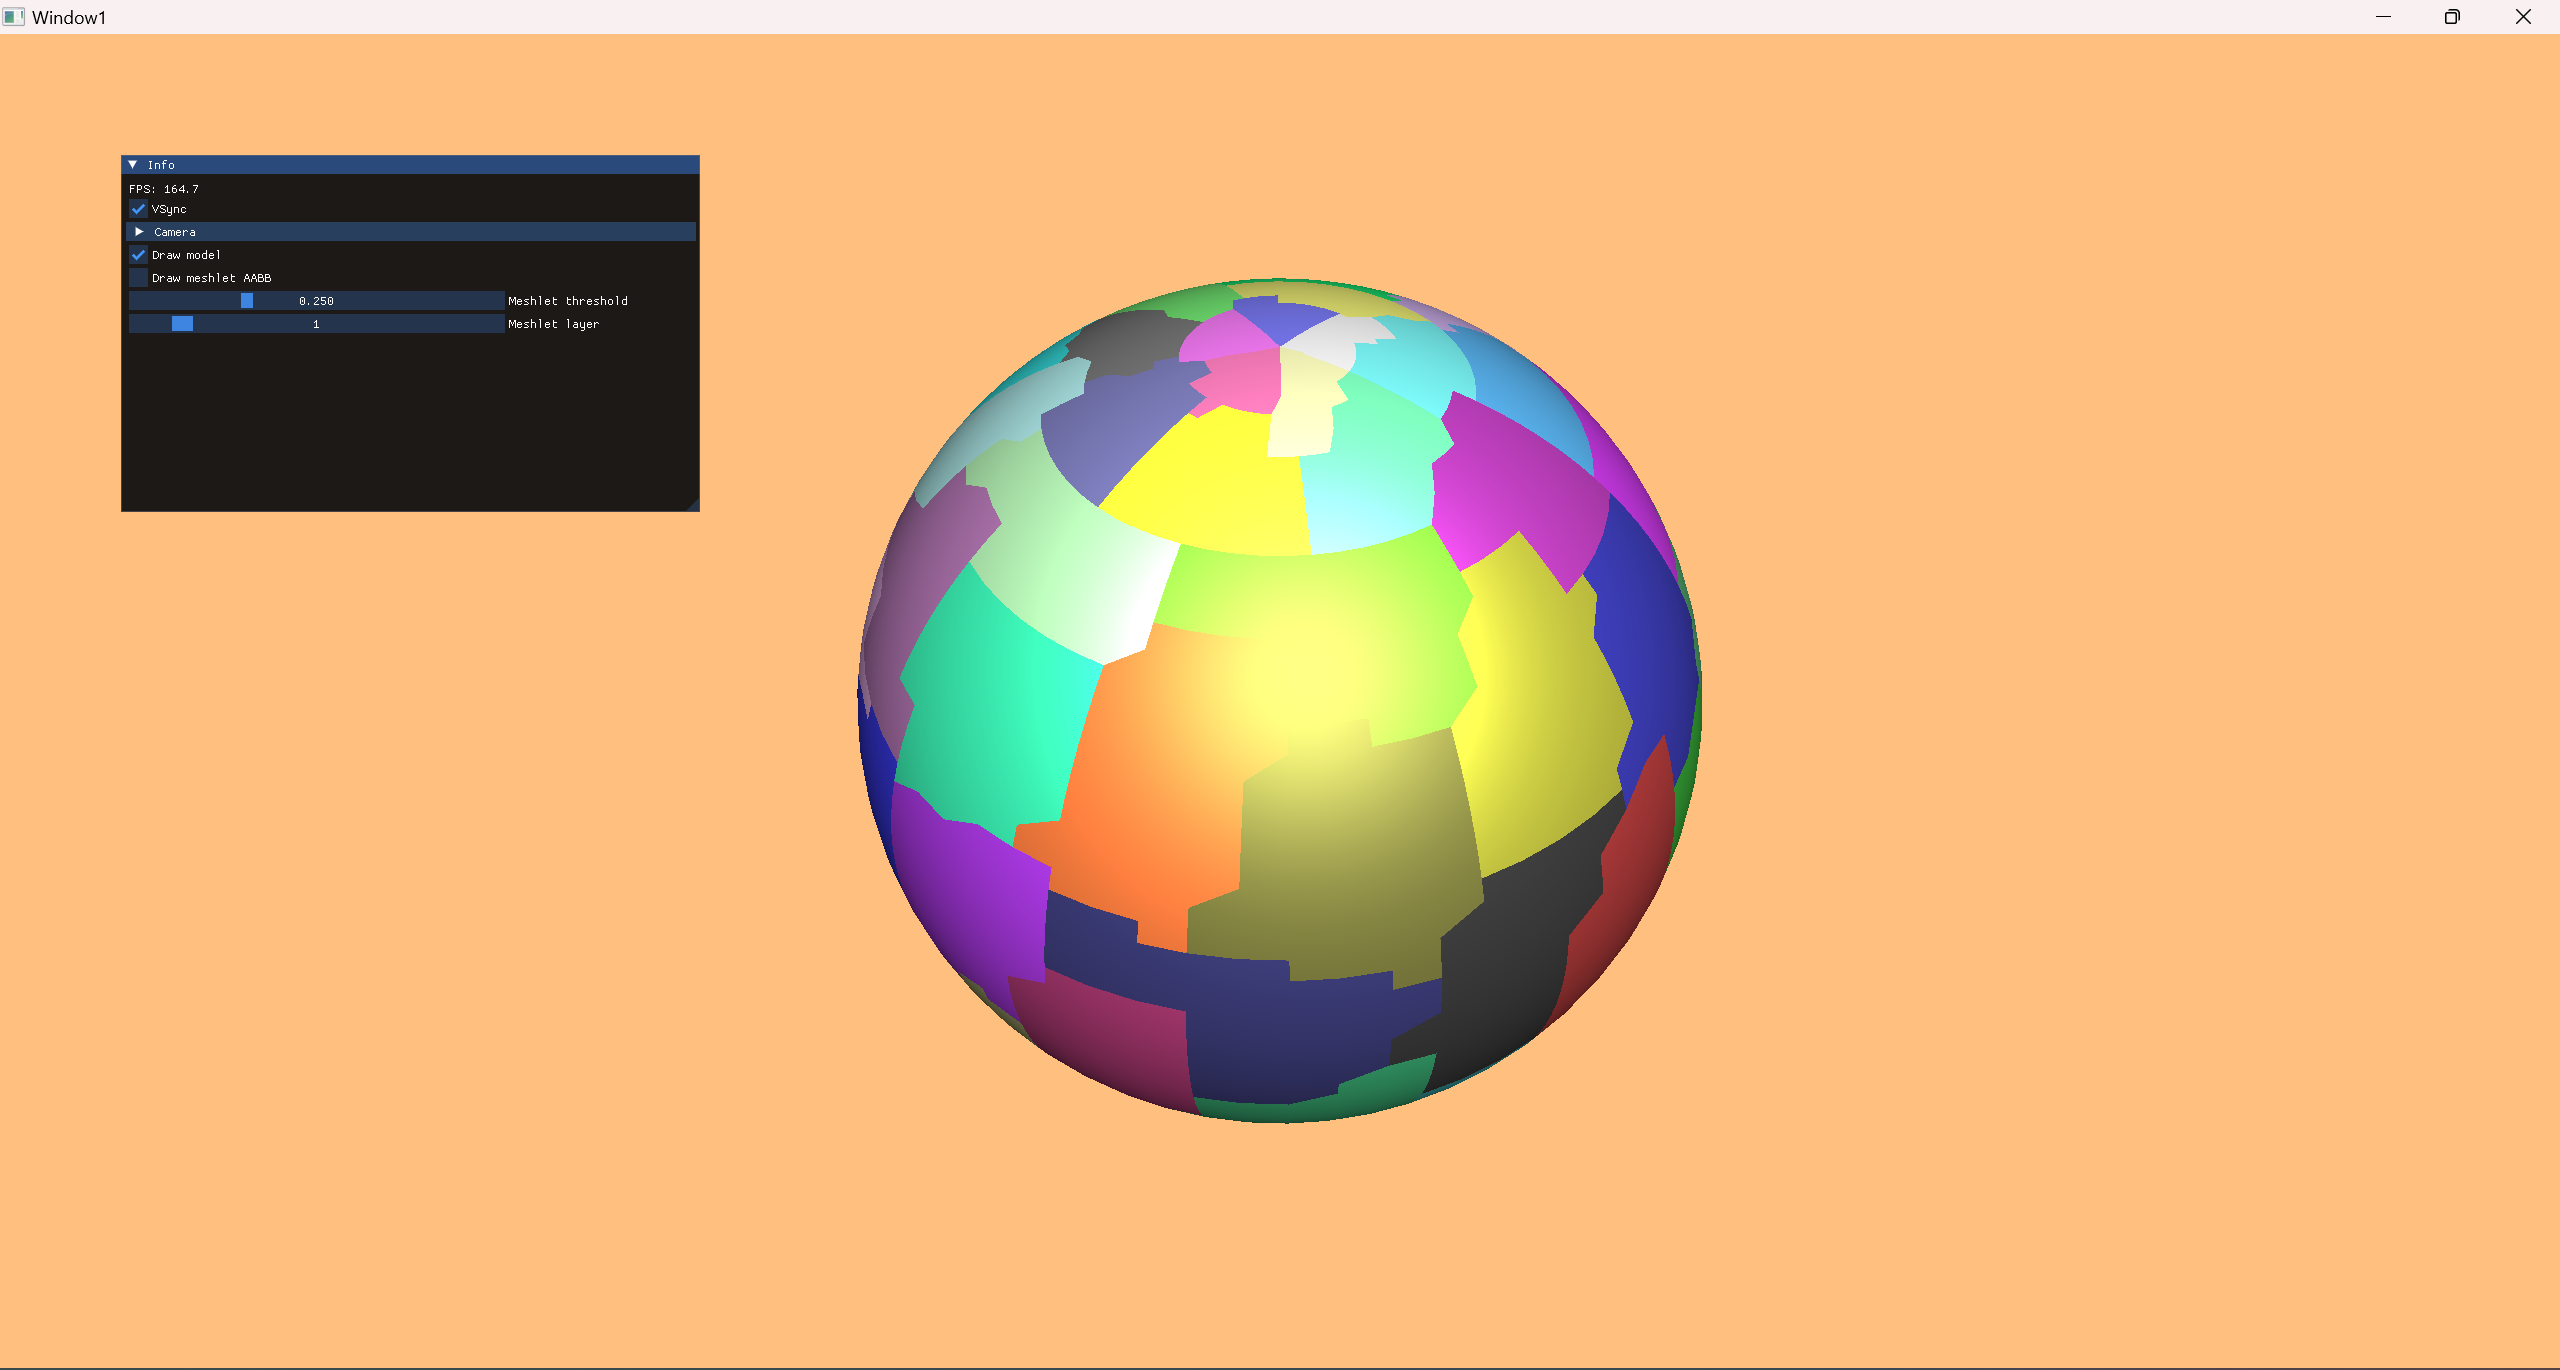
\includegraphics[width=\textwidth]{pics/sphere0.png}
    \caption{Неравномерность разбиения}
    \label{fig:sphere-0}
\end{figure}

Такая неравномерность разбиения, из-за необходимости сохранять швы при децимации, приводит к неравномерности искажений, которые приведены на рисунке~\ref{fig:sphere-1}.
Эта неравномерность искажений может быть заметна глазу при взгляде на изначально симметричные объекты.
\begin{figure}[H]
    \centering
    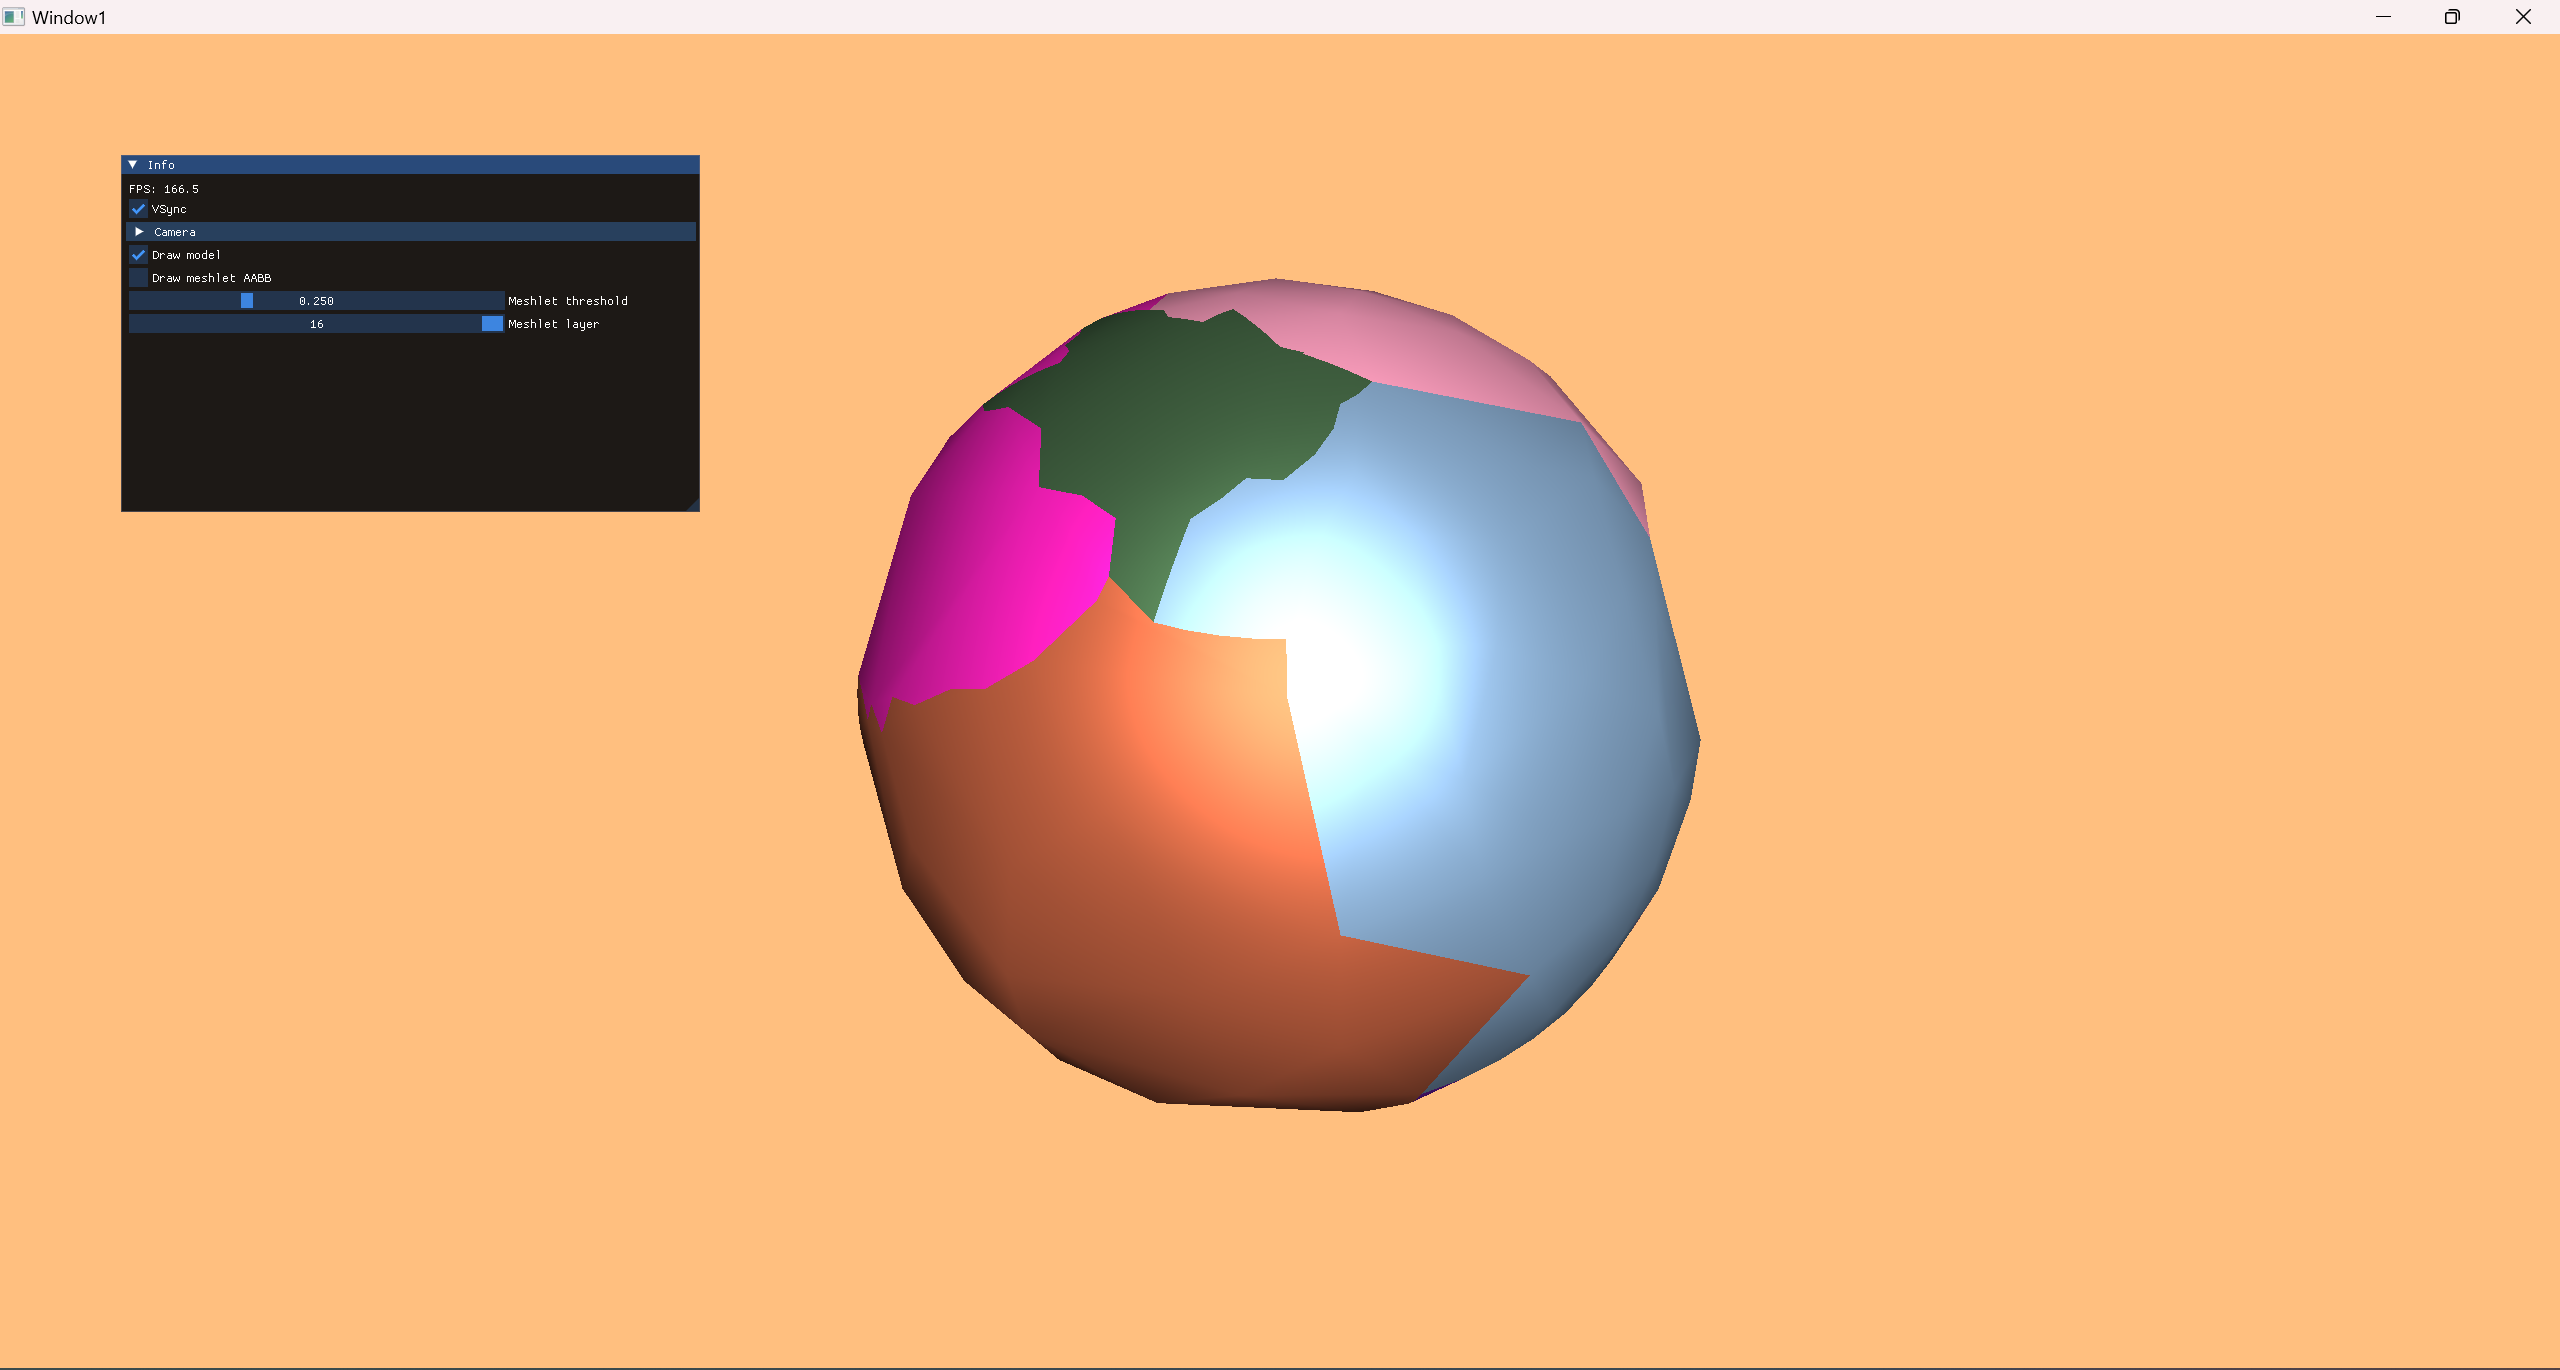
\includegraphics[width=\textwidth]{pics/sphere1.png}
    \caption{Неравномерность искажений}
    \label{fig:sphere-1}
\end{figure}

\subsection*{Ограничение размера мешлетов}
Другой заметной технической проблемой является ограничение размера мешлетов при разбиении графа.
Mesh Shader позволяет использовать мешлеты размером не более 256 вершин и 256 примитивов, это обусловлено механизмом работы общей для группы потоков памяти.
Поскольку METIS не позволяет задать это ограничение, приходится использовать неоптимальное количество мешлетов.

NVidia рекомендует использовать размер мешлета в 64 вершины и 126 треугольников, в то же время размер мешлета на выходе METIS является случайной величиной.

\subsection*{Оптимизация структуры мешлетов}
В ходе реализации было выявлено, что производительность Mesh Shader существенно зависит от организации хранения мешлетов в видеопамяти.
Классический конвейер, оперирующий массивами вершин и индексов жёстко заданных форматов, может оказаться производительнее, чем Mesh Shader, из-за более жёстких ограничений, и, как следствие, более широких возможностей оптимизации.

Так, замена массива вершин и массива индексов на один массив вершин приводит к росту производительности за счёт увеличенного потребления памяти.

AMD также рекомендует~\cite{AMDMeshletsRecommendations} использовать следующие оптимизации:
\begin{itemize}
    \item уменьшать количество вершин, входящих в несколько мешлетов, т.к. такие вершины дублируют вычисления;
    \item уменьшать AABB мешлетов, что позволяет более эффективно отсекать ту геометрию, которая не входит в область видимости;
    \item сжимать массив примитивов так, чтобы следующий примитив использовал индексы предыдущего;
    \item использовать одну из следующих конфигураций:
    \begin{itemize}
        \item до 128 вершин и до 256 треугольников на мешлет, 128 потоков в группе шейдера сетки;
        \item до 64 вершин и до 126 треугольников на мешлет, 64 потока в группе шейдера сетки.
    \end{itemize}
    \item запускать как минимум 32 группы потоков шейдера сетки из одной группы потоков шейдера расширения, чтобы сократить среднее время простоя видеокарты между работой шейдера расширения и шейдера сетки;
    \item минимизировать количество данных, передаваемых между шейдером расширения и шейдером сетки.
\end{itemize}

Как отмечено в презентации, эти оптимизации невозможно провести одновременно, необходимо искать баланс между ними.

\subsection*{Оптимизация отрисовки треугольников}
Как уже было отмечено в главе 1, алгоритмы растеризации, применяемые в видеокартах, всегда запускают пиксельный шейдер хотя бы на квадрате 2 на 2 пикселя, чтобы определить производные промежуточных результатов вычислений по экранным координатам.
Поскольку это в 4 раза увеличивает количество вычислений для треугольников размером 1 пиксель, которых образуется значительное количество, Nanite использует отдельный алгоритм растеризации для обработки этих треугольников.

В рамках выпускной квалификационной работы такой подход было решено не реализовывать ввиду его сложности, но в дальнейших исследованиях необходимо будет исследовать дополнительные алгоритмы растеризации.

\subsection*{Организация параллельного спуска по графу}
Nanite использует персистентный пул потоков вычислительного шейдера на видеокарте вместо запуска одного потока шейдера расширения на каждый мешлет~\cite{KarisNanite}.
Это позволяет Nanite обходить значительно меньшее количество мешлетов, и может существенно повысить производительность отрисовки.

В рамках выпускной квалификационной работы такой подход было решено не реализовывать ввиду его сложности, но в дальнейших исследованиях необходимо будет сравнить персистентный пул потоков с наивным обходом шейдера расширения.

\subsection*{Организация параллельной децимации}
В рамках выпускной квалификационной работы децимация супермешлетов производится в однопоточном режиме.
В результате этого время обработки оказывается значительным: для тестового меша размером 10 млн. треугольников время предподсчёта составило 170 минут на процессоре AMD Ryzen 7 5700H, процессу потребовалось 6 ГБ памяти.

\subsection*{Заключение главы}
В ходе реализации упрощённой версии технологии и при изучении механизма работы Nanite были выявлены следующие технические проблемы, которые необходимо подробнее рассмотреть при реализации полной версии технологии:
\begin{itemize}
    \item задача разбиения графа;
    \item ограничение размера мешлетов;
    \item оптимизация структуры мешлетов;
    \item оптимизация отрисовки треугольников;
    \item организация параллельного спуска по графу;
    \item организация параллельной децимации.
\end{itemize}

В реализованной в выпускной квалификационной работе упрощённой версии технологии некоторые из этих проблем решены частично, для улучшения реализации необходимо дальнейшее их изучение.
